\documentclass[12pt,a4paper]{article}
\usepackage[utf8]{inputenc}
\usepackage{amsmath}
\usepackage{amsfonts}
\usepackage{pdflscape}
\usepackage{amssymb}
\usepackage{array}
\usepackage{graphicx}
\newcolumntype{H}{>{\setbox0=\hbox\bgroup}c<{\egroup}@{}}

\begin{document}
\newpage
Abstract: We test market microstructure invariance of bet hypothesis and its implications using the tick-by-tick transaction data from the Tokyo Stock Exchange (TSE). The pooled regression coefficients of the log of arrival rate on the log of trading activity which range from 0.620 to 0.679 are close to the theoretical value of two-thirds implied by invariance of bet hypothsis. During our sample period, these coefficients vary more cross-sectionally than time-serially suggesting the invariance of bet is affected by different market frictions imposed on different stocks. With the TSE's unique trading features, we calibrate the order-splitting ratios among different minimum tick size groups. The order-splitting ratio of the smallest minimum ticksize group is about 4.17 times of that for the largest minimum ticksize group. However, these order-splitting ratios are close to each other across different volume groups. These findings confirm previous studies that the increase of order-splitting activities due to the market frictions lead to the coefficients deviating from the theoretical value implied by market invariance hypothese.       
\begin{landscape}
\begin{table}[!ht]
\begin{center}
\begin{tabular}{lcccccc}
\multicolumn{7}{c}{Table I: Panel A Descriptive Statstics for All Stocks} \\ \hline
% & (1) & (2) & (3) & (4) & (5) & (6) \\
VARIABLES & N & mean & sd & p1 & p50 & p99 \\ \hline
nprints & 417,297 & 648.976 & 1,398.538 & 2.000 & 194.000 & 6,598.000 \\
avg\_price & 417,297 & 2,003.577 & 2,868.717 & 97.250 & 1,404.952 & 10,082.456 \\
avg\_printsize & 417,297 & 1,024.947 & 27,216.395 & 100.000 & 251.429 & 3,543.902 \\
d\_med\_tw\_size & 417,297 & 164.043 & 2,152.858 & 100.000 & 100.000 & 600.000 \\
d\_med\_vw\_size & 417,297 & 24,578.456 & 851,987.223 & 100.000 & 400.000 & 47,800.000 \\
volatility & 417,297 & 0.017 & 0.010 & 0.004 & 0.015 & 0.054 \\
dollarvol\_in\_1000 & 417,297 & 8,036.155 & 33,074.950 & 3.058 & 629.311 & 125,301.352 \\
\hline
\end{tabular}
\begin{tabular}{lcHcHcHcHcH}
\multicolumn{11}{c}{Panel B: Descriptive Statstics for Ticksize Groups} \\ \hline
% & (1) & (2) & (3) & (4) & (5) & (6) & (7) & (8) & (9) & (10) \\
 & ticksize 1 &  & ticksize 5 &  & ticksize 10 &  & ticksize 50 &  & ticksize 100 &  \\
VARIABLES & mean & N & mean & N & mean & N & mean & N & mean & N \\ \hline
nprints & 591 & 349,074.000 & 768 & 44,110.000 & 1,209 & 23,483.000 & 3,895 & 323.000 & 2,768 & 307.000 \\
avg\_price & 1,283.051 & 349,074.000 & 3,797.550 & 44,110.000 & 7,991.081 & 23,483.000 & 40,742.975 & 323.000 & 64,763.626 & 307.000 \\
avg\_printsize & 1,160.687 & 349,074.000 & 316.201 & 44,110.000 & 360.689 & 23,483.000 & 212.296 & 323.000 & 180.887 & 307.000 \\
d\_med\_tw\_size & 168.675 & 349,074.000 & 125.133 & 44,110.000 & 169.995 & 23,483.000 & 100.000 & 323.000 & 100.000 & 307.000 \\
d\_med\_vw\_size & 28,720.539 & 349,074.000 & 3,531.043 & 44,110.000 & 3,188.153 & 23,483.000 & 292.260 & 323.000 & 672.638 & 307.000 \\
volatility & 0.017 & 349,074.000 & 0.016 & 44,110.000 & 0.016 & 23,483.000 & 0.018 & 323.000 & 0.014 & 307.000 \\
dollarvol\_in\_1000 & 4,646.658 & 349,074.000 & 14,976.849 & 44,110.000 & 36,380.023 & 23,483.000 & 357,454.161 & 323.000 & 329,110.764 & 307.000 \\
N & 349,074& & 44,110& & 23,483& & 323& & 307\\
 \hline
\end{tabular}

\begin{tabular}{lcHcHcHcHcHcHcHcHcHcH}
\multicolumn{21}{c}{Panel C: Descriptive Statstics for Volume Groups} \\ \hline
% & (1) & (2) & (3) & (4) & (5) & (6) & (7) & (8) & (9) & (10) & (11) & (12) & (13) & (14) & (15) & (16) & (17) & (18) & (19) & (20) \\
 &   1 &  &   2 &  &   3 &  &   4 &  &   5 &  &   6 &  &   7 &  &   8 &  &   9 &  &   10 &  \\

VARIABLES & mean & N & mean & N & mean & N & mean & N & mean & N & mean & N & mean & N & mean & N & mean & N & mean & N \\ \hline

nprints & 44 & 124,244.000 & 163 & 84,921.000 & 326 & 41,800.000 & 514 & 41,906.000 & 736 & 20,788.000 & 851 & 20,297.000 & 1,028 & 20,386.000 & 1,344 & 20,681.000 & 1,961 & 21,097.000 & 4,420 & 21,177.000 \\
avg\_price & 1,221.639 & 124,244.000 & 1,435.623 & 84,921.000 & 1,579.472 & 41,800.000 & 1,950.272 & 41,906.000 & 2,163.494 & 20,788.000 & 2,523.116 & 20,297.000 & 2,695.131 & 20,386.000 & 2,903.012 & 20,681.000 & 3,432.067 & 21,097.000 & 6,189.153 & 21,177.000 \\
avg\_printsize & 414.721 & 124,244.000 & 399.514 & 84,921.000 & 437.745 & 41,800.000 & 798.495 & 41,906.000 & 319.544 & 20,788.000 & 523.559 & 20,297.000 & 467.314 & 20,386.000 & 11,112.206 & 20,681.000 & 746.357 & 21,097.000 & 856.631 & 21,177.000 \\
d\_med\_tw\_size & 140.815 & 124,244.000 & 148.865 & 84,921.000 & 164.433 & 41,800.000 & 146.955 & 41,906.000 & 142.332 & 20,788.000 & 205.641 & 20,297.000 & 164.996 & 20,386.000 & 237.029 & 20,681.000 & 229.317 & 21,097.000 & 238.457 & 21,177.000 \\
d\_med\_vw\_size & 2,505.309 & 124,244.000 & 2,279.971 & 84,921.000 & 2,591.859 & 41,800.000 & 27,636.443 & 41,906.000 & 2,064.609 & 20,788.000 & 3,650.505 & 20,297.000 & 4,159.958 & 20,386.000 & 368,216.590 & 20,681.000 & 10,065.915 & 21,097.000 & 21,527.615 & 21,177.000 \\
volatility & 0.014 & 124,244.000 & 0.018 & 84,921.000 & 0.020 & 41,800.000 & 0.020 & 41,906.000 & 0.020 & 20,788.000 & 0.020 & 20,297.000 & 0.018 & 20,386.000 & 0.018 & 20,681.000 & 0.017 & 21,097.000 & 0.016 & 21,177.000 \\
dollarvol\_in\_1000 & 102.094 & 124,244.000 & 465.362 & 84,921.000 & 1,116.658 & 41,800.000 & 2,132.176 & 41,906.000 & 3,482.005 & 20,788.000 & 5,054.238 & 20,297.000 & 7,799.110 & 20,386.000 & 13,009.282 & 20,681.000 & 24,584.997 & 21,097.000 & 96,498.814 & 21,177.000 \\
N &  124,244 & & 84,921& & 41,800 & & 41,906& &20,788 & &20,297 & &20,386 & &20,681 & &21,097 & &21,177\\
 &  &  &  &  &  &  &  &  &  &  &  &  &  &  &  &  &  &  &  &  \\ \hline
\end{tabular}
\end{center}
\end{table}
\end{landscape}
\newpage

\begin{table}
\begin{tabular}{lcccc}
\multicolumn{5}{c}{Table II Pooled Least Square Estimates of Number of Prints} \\ \hline
\multicolumn{5}{c}{$Ln(N_{it}) = \alpha_{0} + \alpha_{1}Ln(\dfrac{W_{it}}{W^{*}}) + \epsilon_{it}$} \\
\multicolumn{5}{c}{$N_{it}$: number of trades for stock i in day t} \\
\multicolumn{5}{c}{$W_{it}$: trading activity -- the product of dollar volume and volatility} \\
\multicolumn{5}{c}{$W^{*}$: benchmark stock trading activity: $601000\times 0.016$} \\
 & (1) & (2) & (3) & (4) \\
VARIABLES & OLS & LSDV & LSDV & LSDV \\ \hline
 &  &  &  &  \\
Log Adj-Trading Activity ($\alpha_{1}$) & 0.679*** & 0.625*** & 0.679*** & 0.620*** \\
 & (0.009) & (0.005) & (0.009) & (0.005) \\
Constant ($\alpha_{0}$) & 5.101*** & 5.103*** & 5.101*** & 5.059*** \\
 & (0.019) & (0.000) & (0.019) & (0.008) \\
 &  &  &  &  \\
Observations & 417,228 & 417,228 & 417,228 & 417,228 \\
Adjusted R-squared & 0.911 & 0.968 & 0.913 & 0.970 \\
Stock FE & NO & YES & NO & YES \\
Day FE & NO & NO & YES & YES \\
 Coef Equal 2/3 p-val & 0.146 & 0.000 & 0.154 & 0.000 \\ \hline
\multicolumn{5}{c}{ Robust (Industry-clustered) standard errors in parentheses} \\
\multicolumn{5}{c}{ *** p$<$0.01, ** p$<$0.05, * p$<$0.1} \\
\end{tabular}
\end{table}

\begin{landscape}
\begin{figure}
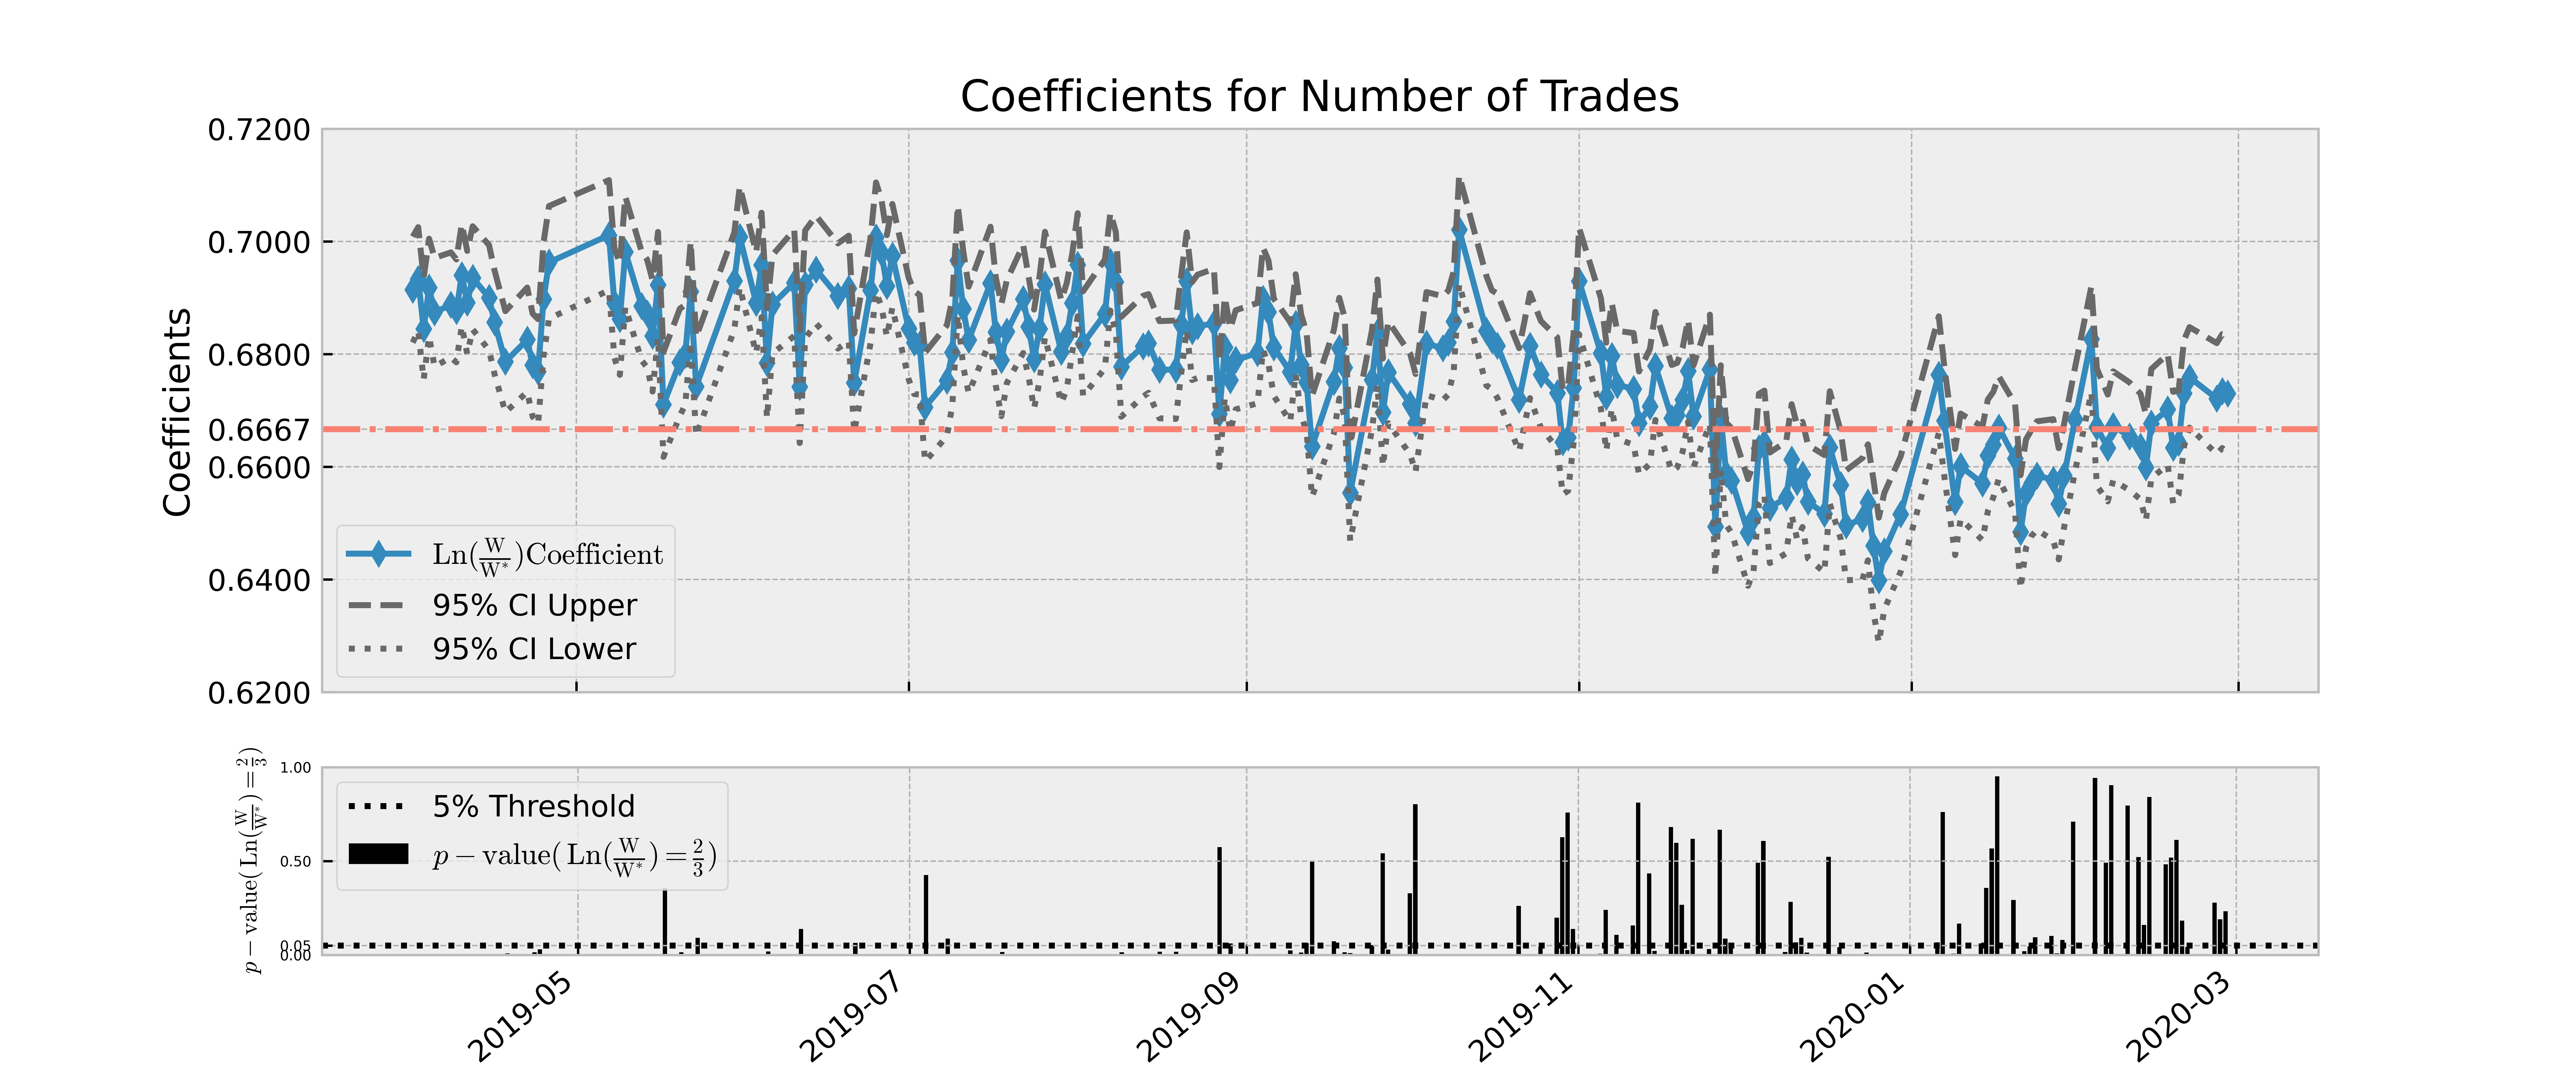
\includegraphics[scale=0.8]{../../times_series_reg_coefficients/res_num_print.jpg} 
\end{figure}
\end{landscape}
\newpage

\begin{landscape}
\begin{table}
\begin{center}
\begin{tabular}{lccccc}
\multicolumn{6}{c}{Table III OLS Estimates of Number of Prints for Ticksize Groups} \\ \hline
\multicolumn{6}{c}{$Ln(N_{it}) = \alpha_{0} + \alpha_{1}Ln(\dfrac{W_{it}}{W^{*}}) + \epsilon_{it}$} \\
 & (1) & (2) & (3) & (4) & (5) \\
VARIABLES & Ticksize 1 & Ticksize 5 & Ticksize 10 & Ticksize 50 & Ticksize 100 \\ \hline
 &  &  &  &  &  \\
Log Adj-Trading Activity ($\alpha_{1}$) & 0.624*** & 0.657*** & 0.638*** & 0.652*** & 0.689*** \\
 & (0.004) & (0.006) & (0.011) & (0.027) & (0.022) \\
Constant ($\alpha_{0}$) & 5.207*** & 4.597*** & 4.424*** & 4.018*** & 3.657*** \\
 & (0.001) & (0.008) & (0.028) & (0.165) & (0.133) \\
 &  &  &  &  &  \\
Observations & 349,005 & 44,110 & 23,483 & 323 & 307 \\
Adjusted R-squared & 0.967 & 0.978 & 0.973 & 0.932 & 0.808 \\
Stock FE & YES & YES & YES & YES & YES \\
Day FE & NO & NO & NO & NO & NO \\
 Coef Equal 2/3 p-val & 0.000 & 0.112 & 0.012 & 0.633 & 0.417 \\ \hline
\multicolumn{6}{c}{ Robust (Industry-clustered) standard errors in parentheses} \\
\multicolumn{6}{c}{ *** p$<$0.01, ** p$<$0.05, * p$<$0.1} \\
\end{tabular}
\end{center}
\end{table}
\end{landscape}







\newpage

\begin{landscape}
\begin{table}
\begin{center}
\footnotesize
\begin{tabular}{lcccccccccc}
\multicolumn{11}{c}{Table IV OLS Estimates of Number of Prints for Volume Groups} \\ \hline
 & (1) & (2) & (3) & (4) & (5) & (6) & (7) & (8) & (9) & (10) \\
VARIABLES & Volume 1 & Volume 2 & Volume 3 & Volume 4 & Volume 5 & Volume 6 & Volume 7 & Volume 8 & Volume 9 & Volume 10 \\ \hline
 &  &  &  &  &  &  &  &  &  &  \\
Log Adj-Trading Activity & 0.618*** & 0.650*** & 0.635*** & 0.623*** & 0.618*** & 0.622*** & 0.620*** & 0.567*** & 0.599*** & 0.585*** \\
 & (0.006) & (0.004) & (0.006) & (0.014) & (0.010) & (0.010) & (0.009) & (0.039) & (0.009) & (0.010) \\
Constant & 4.853*** & 5.129*** & 5.242*** & 5.295*** & 5.328*** & 5.235*** & 5.223*** & 5.311*** & 5.237*** & 5.437*** \\
 & (0.017) & (0.003) & (0.002) & (0.016) & (0.018) & (0.021) & (0.022) & (0.112) & (0.031) & (0.048) \\
 &  &  &  &  &  &  &  &  &  &  \\
Observations & 124,209 & 84,887 & 41,800 & 41,906 & 20,788 & 20,297 & 20,386 & 20,681 & 21,097 & 21,177 \\
Adjusted R-squared & 0.889 & 0.864 & 0.861 & 0.842 & 0.836 & 0.852 & 0.832 & 0.835 & 0.851 & 0.868 \\
Stock FE & YES & YES & YES & YES & YES & YES & YES & YES & YES & YES \\
Day FE & NO & NO & NO & NO & NO & NO & NO & NO & NO & NO \\
 Coef Equal 2/3 p-val & 0.000 & 0.001 & 0.000 & 0.005 & 0.000 & 0.000 & 0.000 & 0.016 & 0.000 & 0.000 \\ \hline
\multicolumn{11}{c}{ Robust standard errors in parentheses} \\
\multicolumn{11}{c}{ *** p$<$0.01, ** p$<$0.05, * p$<$0.1} \\
\end{tabular}
\end{center}
\end{table}
\end{landscape}

\newpage
\begin{landscape}
\begin{table}
\begin{center}
\begin{tabular}{lccccc}
\multicolumn{6}{c}{Table IIIc Restricted Specifications of Number of Prints for Ticksize Groups} \\ 
\multicolumn{6}{c}{Order-splitting Multiplier Calibration} \\
\hline
\multicolumn{6}{c}{$Ln(N_{it}) = Ln(\mu_{0}) + \dfrac{2}{3} Ln(W_{it}) + \epsilon_{it}$} \\
 & (1) & (2) & (3) & (4) & (5) \\
VARIABLES & Ticksize 1 & Ticksize 5 & Ticksize 10 & Ticksize 50 & Ticksize 100 \\ \hline
 &  &  &  &  &  \\
$Ln(\mu_{0})$ & -0.895*** & -1.529*** & -1.766*** & -2.189*** & -2.322*** \\
 & (0.018) & (0.019) & (0.033) & (0.153) & (0.053) \\
 &  &  &  &  &  \\
Observations & 349,005 & 44,110 & 23,483 & 323 & 307 \\
R-squared & 0.924 & 0.945 & 0.928 & 0.860 & 0.735 \\
$\delta_{it}\times \underbrace{(\dfrac{\zeta}{2}E[\dfrac{\zeta}{2}|\tilde{I}|]^{-\dfrac{2}{3}})}_{\text{Constant}}$ & \textbf{0.409} & \textbf{0.217} & \textbf{0.171} & \textbf{0.112} & \textbf{0.098} \\
 rmse & 0.484 & 0.417 & 0.427 & 0.274 & 0.221 \\ \hline
\multicolumn{6}{c}{ Robust standard errors in parentheses} \\
\multicolumn{6}{c}{ *** p$<$0.01, ** p$<$0.05, * p$<$0.1} \\
\end{tabular}

\end{center}
\end{table}
\end{landscape}

\newpage
\begin{landscape}
\begin{table}
\begin{center}
\begin{tabular}{lccccc}
\multicolumn{6}{c}{Table Va Restricted Specifications of Print Size for Ticksize Groups} \\ 
\multicolumn{6}{c}{Order-splitting Multiplier Calibration} \\
\hline
\multicolumn{6}{c}{$Ln(\dfrac{|\tilde{X}_{it}|}{V_{it}}) = Ln(\mu_{x}) - \dfrac{2}{3} Ln(W_{it}) + \epsilon_{it}$} \\
 & (1) & (2) & (3) & (4) & (5) \\
VARIABLES & Ticksize 1 & Ticksize 5 & Ticksize 10 & Ticksize 50 & Ticksize 100 \\ \hline
 &  &  &  &  &  \\
$Ln(\mu_{x})$ & 0.060* & 0.675*** & 0.837*** & 1.449*** & 1.739*** \\
 & (0.032) & (0.033) & (0.051) & (0.269) & (0.124) \\
 &  &  &  &  &  \\
Observations & 349,005 & 44,110 & 23,483 & 323 & 307 \\
$\delta_{it}^{-1} \times \underbrace{E[\dfrac{\zeta}{2}|\tilde{I}|]^{-\dfrac{1}{3}})}_{\text{Constant}}$ & \textbf{1.062} & \textbf{1.963} & \textbf{2.309} & \textbf{4.260} & \textbf{5.690} \\
 rmse & 0.683 & 0.636 & 0.615 & 0.384 & 0.252 \\ \hline
\multicolumn{6}{c}{ Robust standard errors in parentheses} \\
\multicolumn{6}{c}{ *** p$<$0.01, ** p$<$0.05, * p$<$0.1} \\
\end{tabular}
\end{center}
\end{table}
\end{landscape}

\newpage
\begin{landscape}
\begin{table}
\begin{center}
\begin{tabular}{lcccccccccc}
\multicolumn{11}{c}{Table IIIc Restricted Specifications of Number of Prints for Volume Groups} \\ 
\multicolumn{11}{c}{Order-splitting Multiplier Calibration} \\
\multicolumn{11}{c}{$Ln(N_{it}) = Ln(\mu_{0}) + \dfrac{2}{3} Ln(W_{it}) + \epsilon_{it}$} \\\hline
 & (1) & (2) & (3) & (4) & (5) & (6) & (7) & (8) & (9) & (10) \\
VARIABLES & Volume 1 & Volume 2 & Volume 3 & Volume 4 & Volume 5 & Volume 6 & Volume 7 & Volume 8 & Volume 9 & Volume 10 \\ \hline
 &  &  &  &  &  &  &  &  &  &  \\
$Ln(\mu_{0})$ & -1.125*** & -0.975*** & -0.884*** & -0.868*** & -0.869*** & -0.969*** & -1.004*** & -1.093*** & -1.118*** & -1.056*** \\
 & (0.042) & (0.012) & (0.024) & (0.018) & (0.037) & (0.027) & (0.047) & (0.047) & (0.053) & (0.078) \\
 &  &  &  &  &  &  &  &  &  &  \\
Observations & 124,209 & 84,887 & 41,800 & 41,906 & 20,788 & 20,297 & 20,386 & 20,681 & 21,097 & 21,177 \\
$\delta_{it}\times \underbrace{(\dfrac{\zeta}{2}E[\dfrac{\zeta}{2}|\tilde{I}|]^{-\dfrac{2}{3}})}_{\text{Constant}}$ & 0.325 & 0.377 & 0.413 & 0.420 & 0.419 & 0.379 & 0.366 & 0.335 & 0.327 & 0.348 \\
 rmse & 0.629 & 0.475 & 0.446 & 0.462 & 0.466 & 0.509 & 0.470 & 0.607 & 0.526 & 0.582 \\ \hline
\multicolumn{11}{c}{ Robust standard errors in parentheses} \\
\multicolumn{11}{c}{ *** p$<$0.01, ** p$<$0.05, * p$<$0.1} \\
\end{tabular}
\end{center}
\end{table}
\end{landscape}

\newpage
\begin{landscape}
\begin{table}
\begin{center}
\scriptsize
\begin{tabular}{lcccccccc}
\multicolumn{9}{c}{Table V Pooled Least Square Estimates of Quantile Print Sizes} \\ \hline
\multicolumn{9}{c}{$f(Ln(\dfrac{|\tilde{X}_{it}|}{V_{it}})) = \alpha_{0} + \alpha_{1}Ln(\dfrac{W_{it}}{W^{*}}) + \epsilon_{it}$} \\ 
\multicolumn{9}{c}{$\tilde{X}_{it}$ is the print size of a trade for stock i at day t. $f(.)$ is a function (TW or VW) of the 50th percentiles of these distributions. $V_{it}$ is the trading volume for stock i at day t.} \\
 & (1) & (2) & (3) & (4) & (5) & (6) & (7) & (8) \\
VARIABLES & Volume-Weighted & Trade-Weighted & Volume-Weighted & Volume-Weighted & Volume-Weighted & Trade-Weighted & Trade-Weighted & Trade-Weighted \\ \hline
 &  &  &  &  &  &  &  &  \\
Log Adj-Trading Activity ($\alpha_{1}$) & -0.610*** & -0.746*** & -0.501*** & -0.611*** & -0.504*** & -0.705*** & -0.745*** & -0.699*** \\
 & (0.008) & (0.011) & (0.012) & (0.008) & (0.012) & (0.007) & (0.011) & (0.007) \\
Constant ($\alpha_{0}$) & -4.541*** & -5.939*** & -4.546*** & -4.541*** & -4.608*** & -5.941*** & -5.939*** & -5.854*** \\
 & (0.022) & (0.031) & (0.001) & (0.022) & (0.015) & (0.000) & (0.031) & (0.014) \\
 &  &  &  &  &  &  &  &  \\
Observations & 417,228 & 417,228 & 417,228 & 417,228 & 417,228 & 417,228 & 417,228 & 417,228 \\
Adjusted R-squared & 0.761 & 0.885 & 0.850 & 0.770 & 0.859 & 0.965 & 0.887 & 0.967 \\
Stock FE & NO & NO & YES & NO & YES & YES & NO & YES \\
Day FE & NO & NO & NO & YES & YES & NO & YES & YES \\
 Coef Equal -2/3 p-val & 0.000 & 0.000 & 0.000 & 0.000 & 0.000 & 0.000 & 0.000 & 0.000 \\ \hline
\multicolumn{9}{c}{ Robust (Industry-clustered) standard errors in parentheses} \\
\multicolumn{9}{c}{ *** p$<$0.01, ** p$<$0.05, * p$<$0.1} \\
\end{tabular}
\end{center}
\end{table}
\end{landscape}

\newpage
\begin{landscape}
\begin{figure}
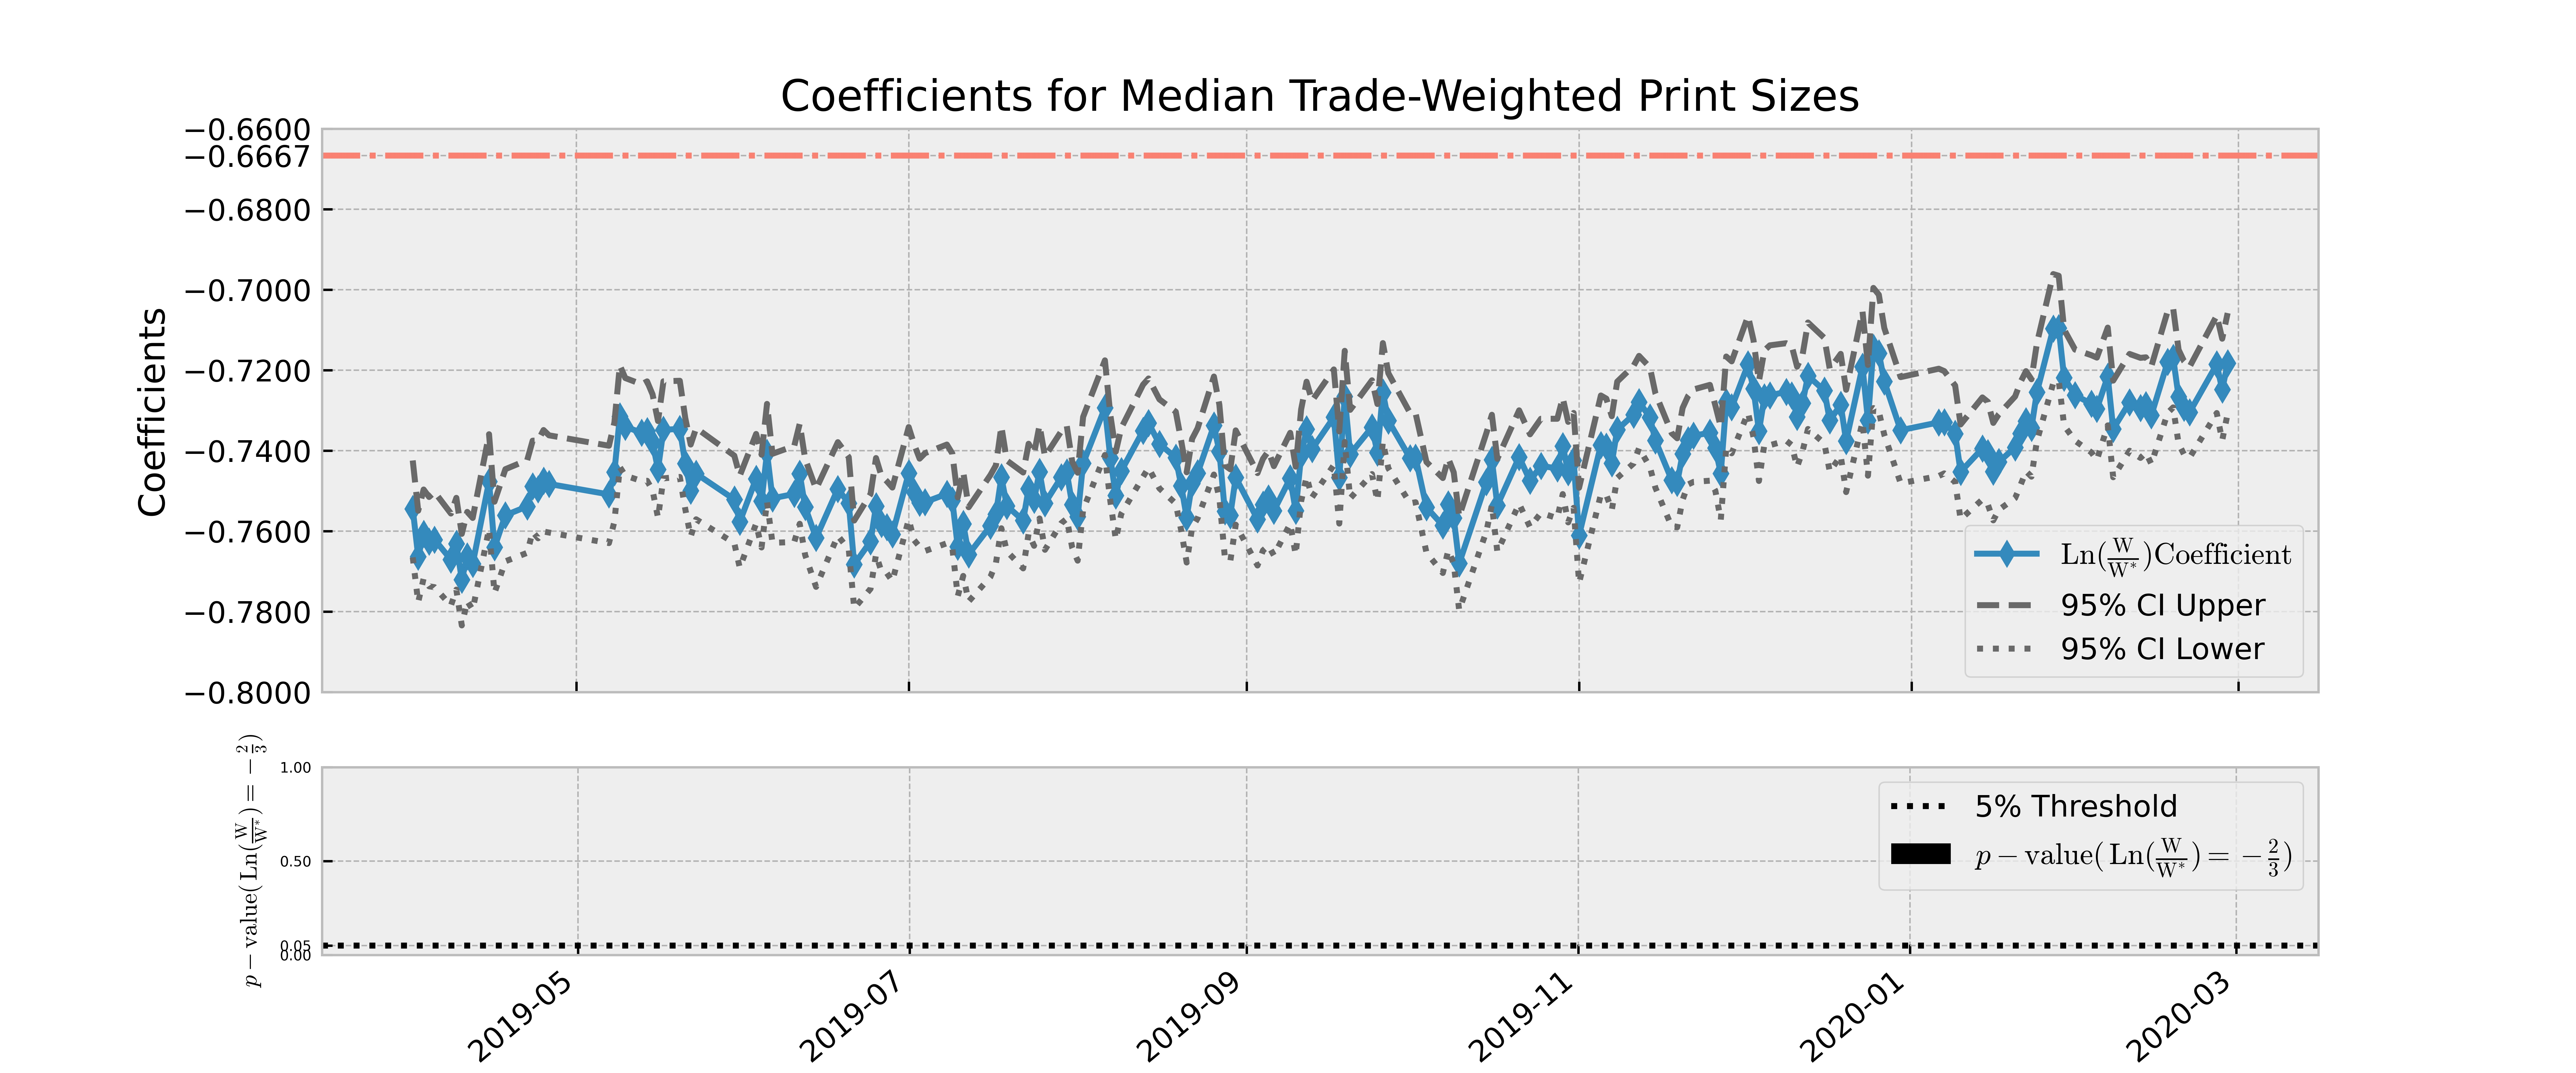
\includegraphics[scale=0.8]{../../times_series_reg_coefficients/res_printsize_tw.jpg} 
\end{figure}
\end{landscape}

\newpage
\begin{landscape}
\begin{figure}
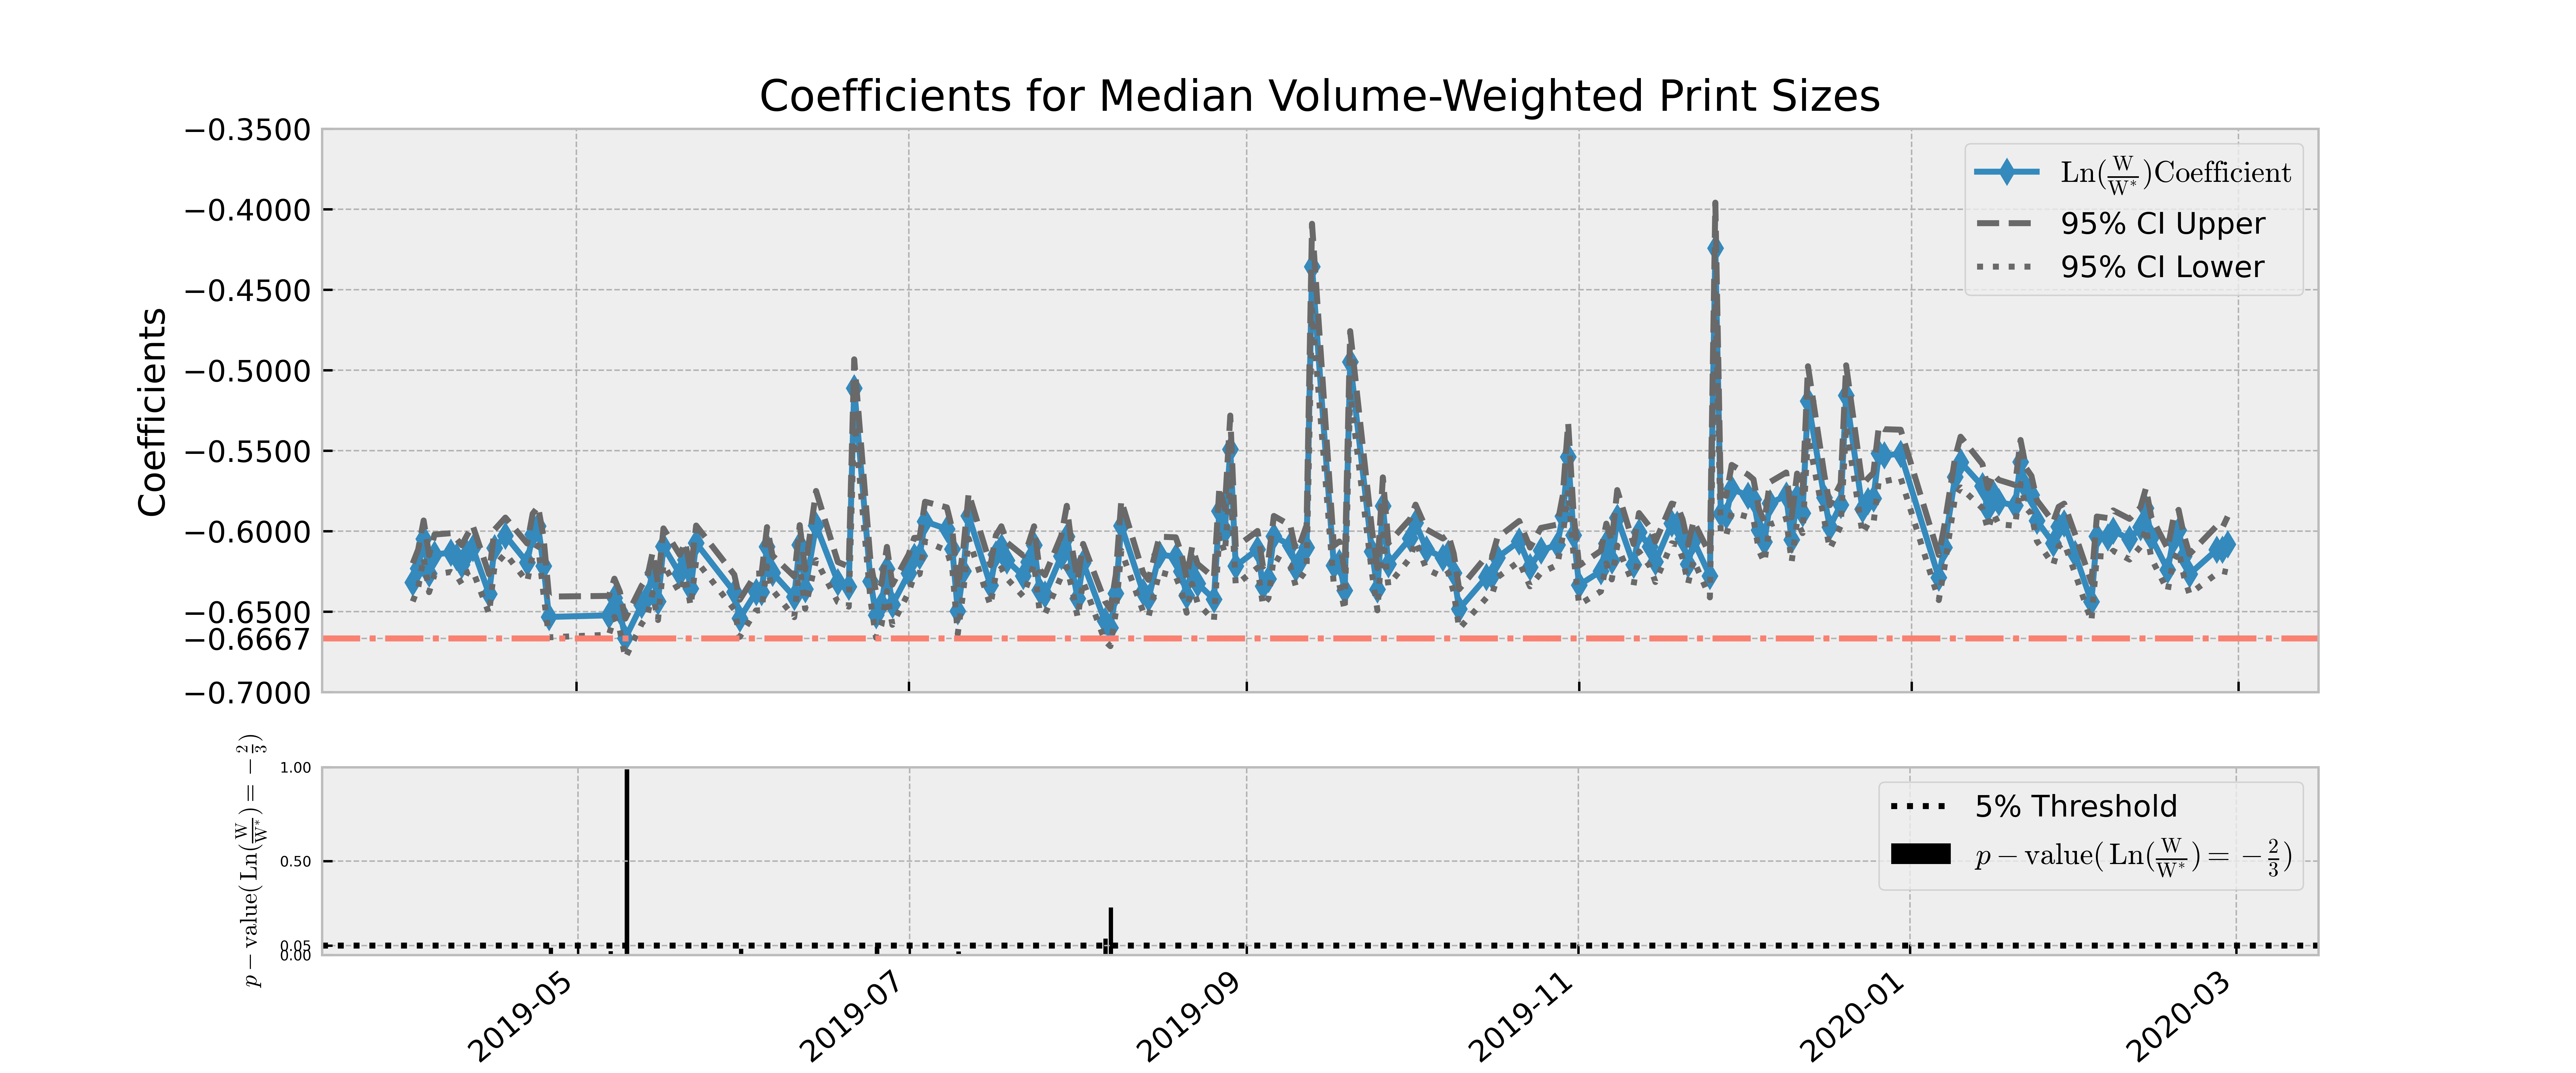
\includegraphics[scale=0.8]{../../times_series_reg_coefficients/res_printsize_vw.jpg} 
\end{figure}
\end{landscape}

\end{document}